\documentclass[12pt,a4paper]{article}

% ===== 中文支持 =====
\usepackage{xeCJK}
\setCJKmainfont{STSong}
\setCJKsansfont{STHeiti}
\setCJKmonofont{STFangsong}

% ===== 页面设置 =====
\usepackage{geometry}
\geometry{left=1in,right=1in,top=1in,bottom=1in}

% ===== 必要宏包 =====
\usepackage{graphicx}
\usepackage{hyperref}
\usepackage{booktabs}
\usepackage{amsmath}
\usepackage{amsfonts}
\usepackage{float}
\usepackage{caption}
\usepackage{tcolorbox}
\usepackage{enumitem}

% ===== 超链接样式 =====
\hypersetup{
    colorlinks=true,
    linkcolor=blue,
    citecolor=blue,
    urlcolor=blue
}

% ===== 自定义命令 =====
\newcommand{\keypoint}[1]{\textbf{核心观点：}#1}
\newcommand{\insight}[1]{\textbf{洞察：}#1}
\newcommand{\suggestion}[1]{\textbf{建议：}#1}
\DeclareMathOperator*{\argmax}{arg\,max}

% ===== 论文信息 =====
\title{\huge Meta-Harness: 模型 Harness 的端到端优化\\[0.5em] \large Meta-Harness: End-to-End Optimization of Model Harnesses}
\author{Yoonho Lee (Stanford) 等\\[0.2cm]\small 导读整理：AI Assistant}
\date{arXiv:2603.28052}

\begin{document}
\maketitle
\begin{abstract}
大语言模型（LLM）系统的性能不仅取决于模型权重，还取决于其 \textit{harness}（控制信息的存储、检索和呈现的代码）。然而，harness 仍主要由手工设计，现有的文本优化器由于过度压缩反馈而不适用于此场景。本文介绍 \textbf{Meta-Harness}，这是一个外环系统，通过端到端搜索来优化 LLM 应用的 harness 代码。它使用一个智能体 proposer，通过文件系统访问所有先验候选的源代码、分数和执行轨迹。在在线文本分类任务上，Meta-Harness 超越最先进的上下文管理系统 7.7 个百分点，同时使用少 4 倍的上下文 token。在检索增强的数学推理上，单个发现的 harness 在 200 个 IMO 级别问题上平均提升 4.7 个百分点。在智能体编码任务上，发现的 harness 超越了最佳手工设计的基线。
\end{abstract}
\tableofcontents
\newpage

% ===== 正文 =====
\section{论文总览}

\subsection{研究背景}

\textbf{Harness 的重要性：} 改变固定大语言模型周围的 harness 可以在同一基准测试上产生 6 倍的性能差距。Harness 是决定存储什么、检索什么以及向模型展示什么的代码，它通常与模型本身一样重要。

\textbf{当前问题：} 尽管 harness 工程很重要，但它仍然是手工的：从业者检查失败案例、调整启发式方法，并在少量设计上进行迭代。本文探索这一过程是否可以自动化。

\subsection{现有方法的局限}

现有的文本优化方法对 harness 工程不匹配，因为它们通常使用\textbf{短视或严重压缩的反馈}：
\begin{itemize}
    \item 仅依赖当前候选或标量分数
    \item 将反馈限制为简短模板或 LLM 生成的摘要
    \item 每个优化步骤的上下文范围仅为 100 到 30,000 token
\end{itemize}

Harness 作用于长视程：关于存储什么、何时检索或如何呈现的单一选择可能会影响许多推理步骤后的行为。压缩的反馈往往会移除追踪下游失败到早期 harness 决策所需的信息。

\subsection{主要贡献}

\begin{enumerate}
    \item \textbf{提出 Meta-Harness：} 一个通过端到端搜索优化 harness 的外环系统，使用智能体 proposer 通过文件系统访问完整的先验经验历史
    \item \textbf{文件系统接口：} 存储所有先验候选的源代码、执行轨迹和分数，proposer 可以通过标准操作（如 grep 和 cat）选择性检索
    \item \textbf{三大任务验证：}
    \begin{itemize}
        \item 在线文本分类：超越 ACE 7.7 个百分点，使用少 4 倍上下文 token
        \item 检索增强数学推理：在 200 个 IMO 级别问题上平均提升 4.7 个百分点
        \item 智能体编码（TerminalBench-2）：超越所有手工设计的 Haiku 4.5 智能体
    \end{itemize}
\end{enumerate}

\section{核心方法}

\subsection{问题定义}

Harness 是一个有状态程序，它包装语言模型并决定模型在每个步骤看到什么上下文。形式化地，令 $M$ 表示固定语言模型，$\mathcal{X}$ 表示任务分布。对于 harness $H$ 和任务实例 $x \sim \mathcal{X}$，执行 rollout 轨迹 $\tau \sim p_M(H, x)$。目标是：

\[
H^* = \argmax_{H} \mathbb{E}_{x \sim \mathcal{X}, \tau \sim p_M(H, x)} \; r(\tau, x)
\]

\subsection{Meta-Harness 搜索循环}

\begin{figure}[h]
    \centering
    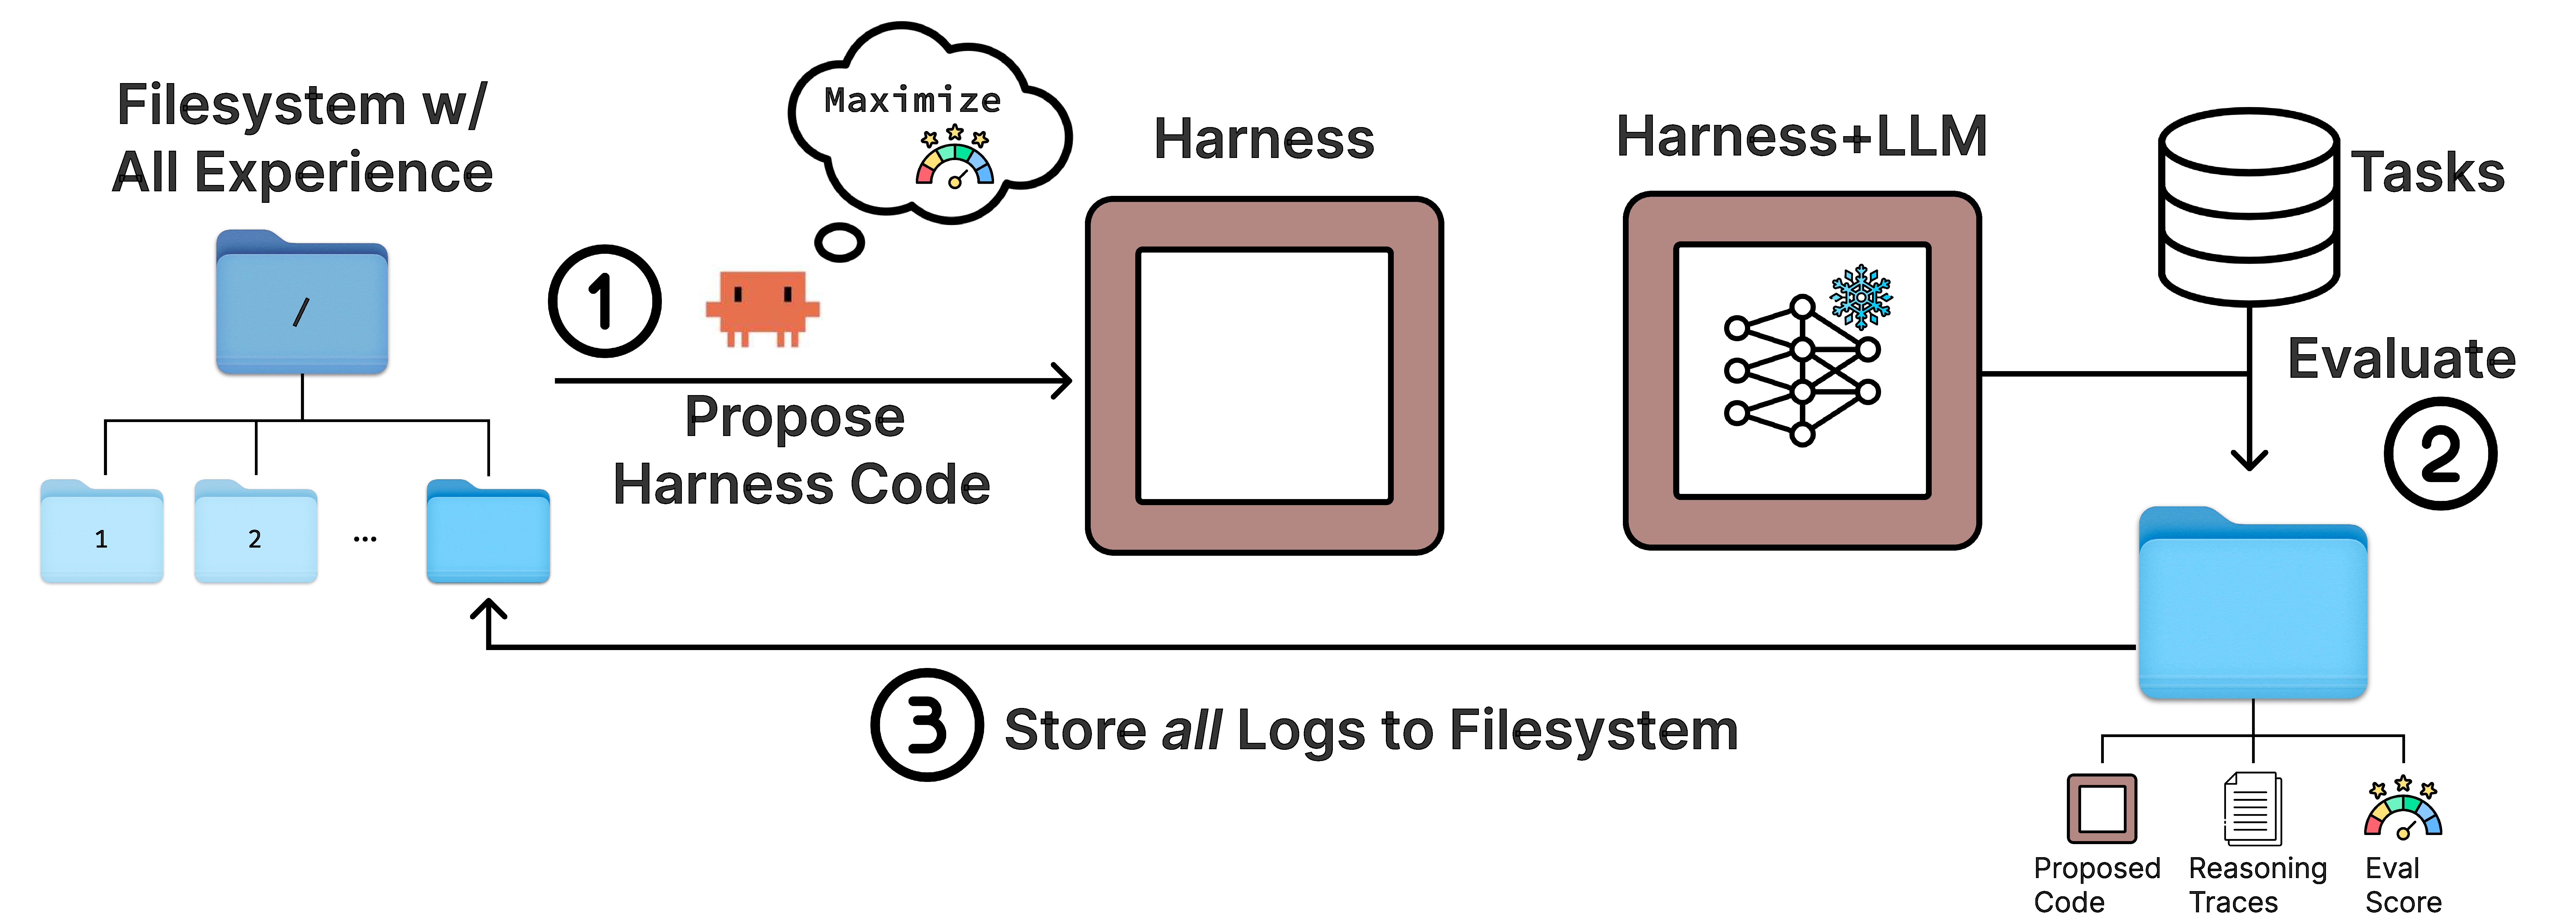
\includegraphics[width=0.9\textwidth]{figures/autoharness_v3.pdf}
    \caption{Meta-Harness 搜索循环。(1) 智能体读取包含所有先验候选源代码、执行轨迹和分数的文件系统，并提出新的 harness；(2) 在评估任务上评估提出的 harness；(3) 所有日志（提出的代码、推理轨迹、评估分数）存储在新目录中，循环重复}
    \label{fig:method}
\end{figure}

\textbf{关键设计：}
\begin{enumerate}
    \item \textbf{Coding Agent Proposer：} 基于语言模型的系统，可以调用开发工具并修改代码
    \item \textbf{完整历史暴露：} 通过文件系统存储所有先验 harness 的源代码、分数和执行轨迹
    \item \textbf{选择性检索：} proposer 通过终端工具（grep、cat）查询文件系统，而非作为单一提示摄入
    \item \textbf{最小结构约束：} 不依赖父代选择规则或预设搜索启发式，proposer 自由检查任何先验 harness
\end{enumerate}

\subsection{代码空间搜索的优势}

\begin{itemize}
    \item \textbf{因果推理：} 通过检查执行轨迹，proposer 可以推断 harness \textit{为什么}失败，以及哪些早期设计决策可能导致失败
    \item \textbf{算法级修改：} proposer 可以修改检索、记忆或提示构造逻辑的算法结构，而非填充模板
    \item \textbf{自然正则化：} 将 harness 表示为程序提供自然正则化偏置，编码模型倾向于提出连贯的算法而非脆弱的硬编码解
\end{itemize}

\section{实验分析}

\subsection{在线文本分类}

\textbf{设置：} 使用 GPT-OSS-120B 作为 LLM 分类器，三个数据集（LawBench、Symptom2Disease、USPTO-50k），20 次迭代产生 40 个候选 harness。

\textbf{对比方法：}
\begin{itemize}
    \item \textbf{文本优化器：} OpenEvolve（进化搜索）、TTT-Discover（PUCT 规则）
    \item \textbf{手工 harness：} ACE（代理上下文工程）、MCE（元上下文工程）
\end{itemize}

\textbf{关键结果：}
\begin{table}[h]
\centering
\caption{在线文本分类主要结果}
\begin{tabular}{lcc}
\toprule
方法 & 准确率 (\%) & 上下文 token (K) \\
\midrule
Zero-shot & 32.1 & 0.1 \\
Few-shot (32) & 38.9 & 12.5 \\
ACE & 40.9 & 50.8 \\
MCE & 40.0 & 28.5 \\
\textbf{Meta-Harness} & \textbf{48.6} & \textbf{11.4} \\
\bottomrule
\end{tabular}
\end{table}

\textbf{核心发现：}
\begin{itemize}
    \item Meta-Harness 在 10 倍更少评估下匹配最佳文本优化器，最终准确率高 10 个百分点
    \item 超越 ACE 7.7 个百分点，同时使用少 4 倍上下文 token
    \item 在 9 个 OOD 数据集上，6 个取得最佳性能
\end{itemize}

\subsection{检索增强数学推理}

\textbf{设置：} 检索 corpus 包含 $\geq$500,000 个已解决问题，在 250 个奥林匹克难度问题上优化 40 次迭代，在 200 个 IMO 级别问题上评估。

\textbf{关键结果：}
\begin{table}[h]
\centering
\caption{数学推理结果（平均准确率 \%) }
\begin{tabular}{lc}
\toprule
方法 & 平均准确率 \\
\midrule
无检索 & 基准 \\
稠密检索 & +0.2 \\
随机 few-shot & +0.5 \\
BM25 检索 & +3.4 \\
\textbf{Meta-Harness} & \textbf{+4.7} \\
\bottomrule
\end{tabular}
\end{table}

\textbf{核心发现：} 单个发现的 harness 在 5 个未见过的模型上泛化，平均提升 4.7 个百分点。

\subsection{TerminalBench-2 智能体编码}

\textbf{设置：} 89 个挑战性任务，需要长视程、完全自主执行。

\textbf{关键结果：}
\begin{itemize}
    \item \textbf{Opus 4.6：} 76.4\% 通过率，超越 Terminus-KIRA (74.7\%)，在所有 Opus 4.5 智能体中排名第 2
    \item \textbf{Haiku 4.5：} 37.6\% 通过率，超越次佳 Goose (35.5\%) 2.1 个百分点，排名第 1
\end{itemize}

\section{关键洞察}

\begin{tcolorbox}[colback=blue!5,colframe=blue!50,title=核心洞察]
\begin{enumerate}
    \item \textbf{完整经验历史的价值：} 文件系统接口使 proposer 能够选择性诊断原始代码和执行轨迹，而非从压缩摘要优化。消融实验证明，仅有分数或分数+摘要的条件远逊于完整执行轨迹访问。
    
    \item \textbf{最小结构偏置：} Meta-Harness 不依赖父代选择规则或预设搜索启发式，这使得它可以自动随 coding agent 能力提升而改进。
    
    \item \textbf{代码空间搜索的可解释性：} 过拟合在代码空间更易检查：脆弱的 if 链或硬编码类映射可通过检查发现，而权重空间的过拟合则不然。
    
    \item \textbf{长视程依赖的关键性：} Harness 工程需要在代码、分数和执行轨迹中分布式的环境反馈，这难以预先总结。
\end{enumerate}
\end{tcolorbox}

\section{实践建议}

\suggestion{对于希望应用类似方法的从业者：}

\begin{enumerate}
    \item \textbf{建立文件系统接口：} 存储所有候选的源代码、执行日志和评估分数，确保 proposer 可以通过命令行工具访问。
    
    \item \textbf{选择强大的 coding agent：} Meta-Harness 使用 Claude Code (Opus-4.6)，coding agent 的能力直接影响搜索质量。
    
    \item \textbf{最小化外环结构：} 避免硬编码搜索启发式，让 proposer 自主决定检查什么、诊断什么以及如何修改。
    
    \item \textbf{关注可解释性：} 定期检查 proposer 的搜索轨迹，理解它如何形成因果假设并修订 harness。
    
    \item \textbf{Pareto 前沿优化：} 同时考虑准确性和上下文成本等多目标，让 proposer 根据期望权衡发现 harness。
\end{enumerate}

\section{局限与未来方向}

\begin{itemize}
    \item \textbf{Proposer 依赖：} 实验仅使用一个强大的 coding agent (Claude Code)，跨不同 proposer 的泛化性有待研究
    \item \textbf{领域覆盖：} 仅在三个领域验证，可能在其他领域的效果不同
    \item \textbf{未来方向：} 协同进化 harness 和模型权重，让策略塑造模型学习内容，反之亦然
\end{itemize}

\section{总结}

\keypoint{Meta-Harness 通过端到端搜索和完整经验历史访问，实现了 harness 工程的自动化。关键创新在于将诊断和提案委托给 coding agent，通过文件系统接口暴露完整历史，使 proposer 能够形成因果假设并针对性修改。实验证明该方法在文本分类、数学推理和智能体编码三个领域均超越手工设计的最佳 harness。}

\begin{tcolorbox}[colback=green!5,colframe=green!50,title=核心引用]
\begin{itemize}
    \item 论文：Meta-Harness: End-to-End Optimization of Model Harnesses
    \item 作者：Yoonho Lee, Roshen Nair, Qizheng Zhang, Kangwook Lee, Omar Khattab, Chelsea Finn
    \item 机构：Stanford, KRAFTON, MIT
    \item arXiv: 2603.28052
    \item 项目页面：\url{https://yoonholee.com/meta-harness/}
\end{itemize}
\end{tcolorbox}

\end{document}
